% Created by tikzDevice version 0.12.6 on 2026-05-14 20:37:34
% !TEX encoding = UTF-8 Unicode
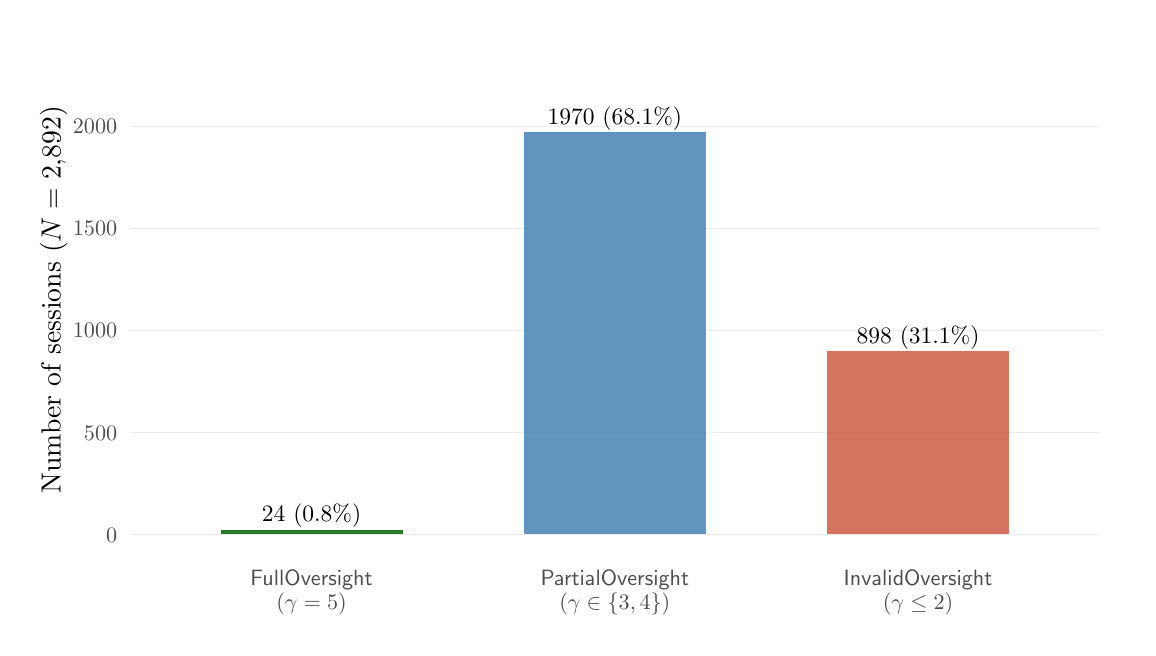
\begin{tikzpicture}[x=1pt,y=1pt]
\definecolor{fillColor}{RGB}{255,255,255}
\path[use as bounding box,fill=fillColor,fill opacity=0.00] (0,0) rectangle (397.48,216.81);
\begin{scope}
\path[clip] (  0.00,  0.00) rectangle (397.48,216.81);
\definecolor{fillColor}{RGB}{255,255,255}

\path[fill=fillColor] (  0.00,  0.00) rectangle (397.48,216.81);
\end{scope}
\begin{scope}
\path[clip] ( 36.83, 25.20) rectangle (387.48,211.81);
\definecolor{drawColor}{gray}{0.92}

\path[draw=drawColor,line width= 0.5pt,line join=round] ( 36.83, 33.69) --
	(387.48, 33.69);

\path[draw=drawColor,line width= 0.5pt,line join=round] ( 36.83, 70.57) --
	(387.48, 70.57);

\path[draw=drawColor,line width= 0.5pt,line join=round] ( 36.83,107.44) --
	(387.48,107.44);

\path[draw=drawColor,line width= 0.5pt,line join=round] ( 36.83,144.32) --
	(387.48,144.32);

\path[draw=drawColor,line width= 0.5pt,line join=round] ( 36.83,181.20) --
	(387.48,181.20);
\definecolor{fillColor}{RGB}{0,100,0}

\path[fill=fillColor,fill opacity=0.85] ( 69.70, 33.69) rectangle (135.45, 35.46);
\definecolor{fillColor}{RGB}{70,130,180}

\path[fill=fillColor,fill opacity=0.85] (179.28, 33.69) rectangle (245.03,178.99);
\definecolor{fillColor}{RGB}{205,91,69}

\path[fill=fillColor,fill opacity=0.85] (288.86, 33.69) rectangle (354.61, 99.92);
\definecolor{drawColor}{RGB}{0,0,0}

\node[text=drawColor,anchor=base,inner sep=0pt, outer sep=0pt, scale=  0.85] at (102.58, 38.40) {24 (0.8\%)};

\node[text=drawColor,anchor=base,inner sep=0pt, outer sep=0pt, scale=  0.85] at (212.16,181.93) {1970 (68.1\%)};

\node[text=drawColor,anchor=base,inner sep=0pt, outer sep=0pt, scale=  0.85] at (321.74,102.86) {898 (31.1\%)};
\end{scope}
\begin{scope}
\path[clip] (  0.00,  0.00) rectangle (397.48,216.81);
\definecolor{drawColor}{gray}{0.30}

\node[text=drawColor,anchor=base east,inner sep=0pt, outer sep=0pt, scale=  0.80] at ( 32.33, 30.93) {0};

\node[text=drawColor,anchor=base east,inner sep=0pt, outer sep=0pt, scale=  0.80] at ( 32.33, 67.81) {500};

\node[text=drawColor,anchor=base east,inner sep=0pt, outer sep=0pt, scale=  0.80] at ( 32.33,104.69) {1000};

\node[text=drawColor,anchor=base east,inner sep=0pt, outer sep=0pt, scale=  0.80] at ( 32.33,141.57) {1500};

\node[text=drawColor,anchor=base east,inner sep=0pt, outer sep=0pt, scale=  0.80] at ( 32.33,178.45) {2000};
\end{scope}
\begin{scope}
\path[clip] (  0.00,  0.00) rectangle (397.48,216.81);
\definecolor{drawColor}{gray}{0.30}

\node[text=drawColor,anchor=base,inner sep=0pt, outer sep=0pt, scale=  0.80] at (102.58, 15.20) {$\mathsf{FullOversight}$};

\node[text=drawColor,anchor=base,inner sep=0pt, outer sep=0pt, scale=  0.80] at (102.58,  6.56) {($\gamma=5$)};

\node[text=drawColor,anchor=base,inner sep=0pt, outer sep=0pt, scale=  0.80] at (212.16, 15.20) {$\mathsf{PartialOversight}$};

\node[text=drawColor,anchor=base,inner sep=0pt, outer sep=0pt, scale=  0.80] at (212.16,  6.56) {($\gamma \in \{3,4\}$)};

\node[text=drawColor,anchor=base,inner sep=0pt, outer sep=0pt, scale=  0.80] at (321.74, 15.20) {$\mathsf{InvalidOversight}$};

\node[text=drawColor,anchor=base,inner sep=0pt, outer sep=0pt, scale=  0.80] at (321.74,  6.56) {($\gamma \leq 2$)};
\end{scope}
\begin{scope}
\path[clip] (  0.00,  0.00) rectangle (397.48,216.81);
\definecolor{drawColor}{RGB}{0,0,0}

\node[text=drawColor,rotate= 90.00,anchor=base,inner sep=0pt, outer sep=0pt, scale=  1.00] at ( 11.89,118.51) {Number of sessions ($N = 2{,}892$)};
\end{scope}
\end{tikzpicture}
